\documentclass[runningheads]{llncs}


\usepackage{tikz}
\usepackage{calc}
\usepackage{amsmath,amssymb}
\usetikzlibrary{automata}

\DeclareMathOperator*{\argmin}{arg\,min}

\usepackage{wasysym}




\begin{document}

\title{On finiteness of structures produced deterministically by co-transcriptional folding}

\section{Infiniteness of delay-1 unary deterministic oritatami system}

\begin{figure}
  \begin{center}
    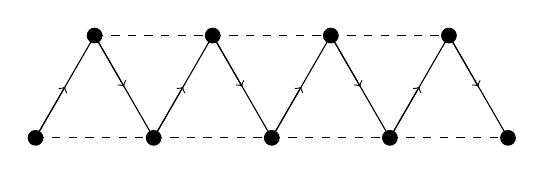
\begin{tikzpicture}
      \fill (0,0) circle[radius = 0.1];
      \fill (1.5,0) circle[radius = 0.1];
      \fill (3,0) circle[radius = 0.1];
      \fill (4.5,0) circle[radius = 0.1];
      \fill (6,0) circle[radius = 0.1];

      \draw[dashed] (0,0)--(1.5,0);
      \draw[dashed] (1.5,0)--(3,0);
      \draw[dashed] (3,0)--(4.5,0);
      \draw[dashed] (4.5,0)--(6,0);
      \draw[->] (0,0)--(60:0.75);
      \draw[->] (1.5,0)--++(60:0.75);
      \draw[->] (3,0)--++(60:0.75);
      \draw[->] (4.5,0)--++(60:0.75);
      \draw (0,0)--(60:1.5);
      \draw (1.5,0)--++(60:1.5);
      \draw (3,0)--++(60:1.5);
      \draw (4.5,0)--++(60:1.5);
      
      \begin{scope}[shift=(60:1.5)]
        \fill (0,0) circle[radius = 0.1];
        \fill (1.5,0) circle[radius = 0.1];
        \fill (3,0) circle[radius = 0.1];
        \fill (4.5,0) circle[radius = 0.1];
        \draw[dashed] (0,0)--(1.5,0);
        \draw[dashed] (1.5,0)--(3,0);
        \draw[dashed] (3,0)--(4.5,0);
        \draw[->] (0,0)--(-60:0.75);
        \draw[->] (1.5,0)--++(-60:0.75);
        \draw[->] (3,0)--++(-60:0.75);
        \draw[->] (4.5,0)--++(-60:0.75);
        
        \draw (0,0)--(-60:1.5);
        \draw (1.5,0)--++(-60:1.5);
        \draw (3,0)--++(-60:1.5);
        \draw (4.5,0)--++(-60:1.5);
      \end{scope}
      
    \end{tikzpicture}
    \caption{zig-zag conformation}
    \label{TTT_zigzag}
  \end{center}
\end{figure}

\subsection{Introduction}


In this section, we consider the finiteness of structures produced deterministically at delay 1. Our result, cases of arity 1 and 3 can only yield finite structures of size $\mathcal{O} (n)$, and cases of arity 4 and more can only yield finite structures which is size of $mathcal{O} (n^2)$, and a case of arity 2 can yield infinite structures but they are only the zig-zag conformation shown in Fig.\ref{TTT_zigzag}. 

%In this section, we prove that unary oritatami system can form infinitely at delay 1 and arity 2 deterministically and moreover that the only infinite conformations which its oritatami system can yield is only the zig-zag conformation shown in Fig.\ref{TTT_zigzag}. 


Let $\Xi$ be a deterministic oritatami system of delay 1 and arity 2. Assume its seed $\sigma$ consists of $n$ beads.
%Let us denote its transcript by $w = w_1 w_2 w_3 \cdots$ for some $w_1,w_2,w_3 \in \Sigma = \{e\}$.
For $i \geq 0$ let $C_i$ be the unique elongation of $\sigma$ by $w[1..i]$, that is, foldable by $\Xi$. Hence $C_0 = \sigma$.


Let us consider the stabilization of the $i$-th bead $a_i$ upon $C_{i-1}$. The bead cannot collaborate with any succeeding bead $w[i+1],w[i+2],\cdots$ at delay 1. There are just two ways to get stabilized at delay 1. One way is to be bound to another bead. The other way is through a $tunnel\ section$. A tunnel section consists of four beads that occupy four neighbors of a point (Fig.\ref{TTT_tunnel_intro}). 
Accordingly, how they are stabilized can be described by a binary sequence $S$ of $b$'s (bound) and $t$'s (tunnel section); priority is given to $t$, that is, $S[i] = t$ if the $i$-th bead $w_i$ is stabilized not only by being bound but also through a tunnel section. 

Assume that four of the six neighbors of a point $p$ are occupied by beads $a_{j_1},a_{j_2},a_{j_3},a_{j_4}$ while the other two are free. We call such a point $p$ the $inside\ of\ a\ tunnel$ and points $p^\prime$ the $entrance\ of\ a\ tunnel$ except when $p^\prime$ is inside of a tunnel. If the beads $w[i-2]$ and $w[i-1]$ are stabilized respectively at one of the two free neighbors and at $p$ one after another, then the next bead $w[i]$ cannot help but be stabilized at the other free neighbor. In this way, $w[i]$ can get stabilized without being bound.

%If a bead is stabilized through a tunnel section, then it can provide some bonds. Let us consider bonds of $C_i$. $C_i$ is represented $C = (W,P,H)$ where $|W| = i + n$ $C_i$ contains $\alpha \cdot (i + n) - 2|H|$ bonds because $C_i$ consists of $i + n$ beads and a bead has just $\alpha$ bonds and then $2 |H|$ of the those bonds are already used. However, even if a bead has an available bond, $w[j]$ $(j > i)$ might not be able to use this bond because the bond has possibility that it is blocked by transcripts $w[i+1..j-1]$. Number of $binding\ capabilities$ does not contain that case so that it is at most $\alpha \cdot (i + n) - 2|H|$.

We say that point $p$ is reachable from a conformation $C$ if there exists a directed path $P^\prime$ from the last point of $C$ that does not cross the path of $C$. We define $binding\ capability$ with reachable.

\begin{definition}[binding capability]
Let $B_i$ be $( \{ (h, i) | {}^\forall h < i \} \cup \{ (i, j) | {}^\forall j > i \}) \cap H$. Moreover, let $R_i$ be a set of neighbors of $w[i]$ that are free and reachable from $C_j$ where $C_j$ is a conformation which stabilized until $w[j]$.
 The number of binding capabilities of a conformation $C_j$ is denoted $\#bc(C_j)$ and is defined by $\sum^{j}_{k=-n+1} \min \{ |B_k|, |R_k|  \}$.
\end{definition}


\begin{figure}
  \begin{center}
    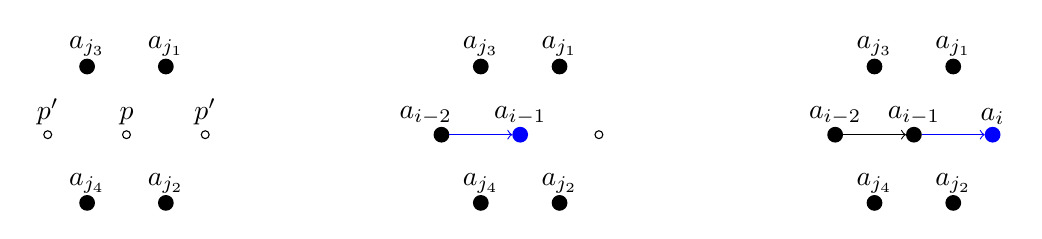
\begin{tikzpicture}
      \draw (0:0) circle [radius=0.05];
      \draw (0:1) circle [radius=0.05];
      \draw (180:1) circle [radius=0.05];
      \node[above] at (0:1) { $p^\prime$ };
      \node[above] at (0:0) { $p$ };
      \node[above] at (180:1) { $p^\prime$ };
      
      \fill (60 : 1) circle [radius=0.1];
      \fill (-60 : 1) circle [radius=0.1];
      \fill (120 : 1) circle [radius=0.1];
      \fill (-120 : 1) circle [radius=0.1];
      \node[above] at (60 :1) { $a_{j_1}$ };
      \node[above] at (-60 :1) { $a_{j_2}$ };
      \node[above] at (120 :1) { $a_{j_3}$ };
      \node[above] at (-120 :1) { $a_{j_4}$ };
      
      \begin{scope}[shift=(0:5)]
        \fill[blue] (0:0) circle [radius=0.1];
        \draw (0:1) circle [radius=0.05];
        \fill (180:1) circle [radius=0.1];
        \node[above] at (180:1.2) { $a_{i-2}$ };
        \node[above] at (0:0) { $a_{i-1}$ };
        \draw[->, blue] (180:0.9) -- (180:0.1);
        
        \fill (60 : 1) circle [radius=0.1];
        \fill (-60 : 1) circle [radius=0.1];
        \fill (120 : 1) circle [radius=0.1];
        \fill (-120 : 1) circle [radius=0.1];
        \node[above] at (60 :1) { $a_{j_1}$ };
        \node[above] at (-60 :1) { $a_{j_2}$ };
        \node[above] at (120 :1) { $a_{j_3}$ };
        \node[above] at (-120 :1) { $a_{j_4}$ };
      \end{scope}
      \begin{scope}[shift=(0:10)]
        \fill (0:0) circle [radius=0.1];
        \fill[blue] (0:1) circle [radius=0.1];
        \fill (180:1) circle [radius=0.1];
        \node[above] at (180:1) { $a_{i-2}$ };
        \node[above] at (0:0) { $a_{i-1}$ };
        \node[above] at (0:1) { $a_i$ };
        \draw[->] (180:0.9) -- (180:0.1);
        \draw[->,blue] (0:0.1) -- (0:0.9);
        
        \fill (60 : 1) circle [radius=0.1];
        \fill (-60 : 1) circle [radius=0.1];
        \fill (120 : 1) circle [radius=0.1];
        \fill (-120 : 1) circle [radius=0.1];
        \node[above] at (60 :1) { $a_{j_1}$ };
        \node[above] at (-60 :1) { $a_{j_2}$ };
        \node[above] at (120 :1) { $a_{j_3}$ };
        \node[above] at (-120 :1) { $a_{j_4}$ };
      \end{scope}
    \end{tikzpicture} 
    \caption{Through a tunnel section}
    \label{TTT_tunnel_intro}
  \end{center}
\end{figure}




\begin{theorem}[Tunnel Troll Theorem]
Let $\Xi$ be a unary oritatami system of $\delta = 1, \alpha = 2$. If there are indices $i$ and $j$ such that $S[i..j+1] = bbt^{(j-i-1)}b$, then $\#bc(C_{i-1}) > \#bc(C_j)$ and if $S[i..j+1] = bt^lbt^mb \quad (l + m = j-i-1)$, then $\#bc(C_{i-1}) > \#bc(C_j)$. On the other hand, at $\delta = 1$ and $\alpha \geq 3$, if S$[k] = t$, then $\#bc(C_{k-1}) > \#bc(C_k)$.
\end{theorem}

%%%%%%%%%%%%%%%%%%%%%%%%%%%%%%%%%%%%%%%%%%%%%%%%%%%%


\proof%{Proof of Tunnel Troll Theorem}
Assume $\Xi$ is deterministic.
Each bead in the transcript is bound either inside a tunnel or outside. If a bead is stabilized inside a tunnel, then the position of successor is already decided either inside of a tunnel or outside. Moreover, if a bead is stabilized outside a tunnel, then its position is either an entrance of a tunnel or not.

Tunnel sections have three possible shapes up to symmetry : straight($A$), obtuse($B$) and acute($C$) turn (Fig. \ref{TTT_tunnel}), and we will consider each of those. 

\begin{lemma}
\label{TTT_neighbor_lemma}
For unary transcripts at $\delta = 1$, if a bead has no free hand, then at least $\alpha + 2$ of its neighbors have to be occpied.
\end{lemma}

\begin{lemma}
\label{TTT_entrance_Tab}
Let $\Xi$ be an oritatami system at $\delta = 1, \alpha =2$. 
Assume $\Xi$ stabilizes the transcript until $w[i-1]$. If $w[i]$ is stabilized at an entrance point of tunnel $A$ or $B$, then $\#bc(C_{i-1}) > \#bc(C_{i})$.
\end{lemma}

\begin{lemma}
\label{TTT_exit}
Let $w[i]$ be a bead which is stabilized at the exit of a tunnel.
At $\delta = 1, \alpha =2$, if we assume $S[h..i+1] = bt^{(i-h)}b \quad (h<i)$, then $\#bc(C_{h-1}) \geq \#bc(C_i)$ and $\#bc(C_{i-2}) \geq \#bc(C_i)$.
%if we assume $\#bc(C_{i-2}) - \#bc(C_{i-1}) = a$, then $\#bc(C_{i}) - \#bc(C_{i-1}) \leq a$.
On the other hand, if we assume $S[k] = t (k \leq i)$ at $\delta =1, \alpha \geq 3$, then $\#bc(C_{k-1}) > \#bc(C_{k})$.
\end{lemma}

\begin{lemma}
\label{TTT_tunnelC_lemma}
Let $\Xi$ be a unary oritatami system of $\delta = 1, \alpha = 2$. We assume $S[h..i+1] = bt^{(i-h)}b \quad (1<h<i)$. If at least one of $w[h+1..i]$ is stabilized by tunnel $C$, then $\#bc(C_{h-3}) > \#bc(C_{h+1})$ and $\#bc(C_{h-3}) > \#bc(C_i)$.
\end{lemma}


Let us first consider cases of $\delta \geq 3, \alpha = 1$. These cases are clearly true because of lemma\ref{TTT_exit}.


Next, we consider the case of $\delta = 2, \alpha = 1$. We assume there is an index $h$ such that $S[h-1..h+1] = bbt$ or $S[h-1..h+1] = tbt$. According to lemma\ref{TTT_entrance_Tab}, if $w[h+1]$ is stabilized by tunnel $A$ or $B$, then $\#bc(C_{h-1}) > \#bc(C_{h})$. Also,  According to lemma\ref{TTT_tunnelC_lemma}, if $w[h+1]$ is stabilized by tunnel $C$, then $\#bc(C_{h-3}) > \#bc(C_{h+1})$.
On the other hand, if $S[k..l] = bt^{l-k}b$, then $\#bc(C_{k-1}) \geq \#bc(C_{l})$ because of lemma\ref{TTT_exit}. Therefore, if there are indices $i$ and $j$ such that $S[i..j+1] = bbt^{(j-i-1)}b$ or $S[i..j+1] = bt^mbt^nb \quad (m + n = j-i-1)$, then $\#bc(C_{i-1}) > \#bc(C_{j})$.

\qed

\begin{figure}
  \begin{center}
    \begin{tabular}{ccc}
      
      \begin{minipage}{0.3\hsize}
        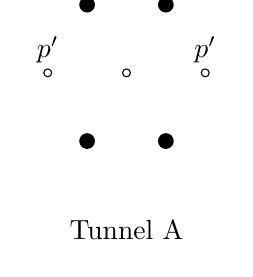
\begin{tikzpicture}
          \begin{scope}[xshift=2cm, yshift=2cm]
            \draw(0,0) circle [radius=0.05];
            \node[above] at (180:1) {$p^\prime$};
            \node[above] at (0:1) {$p^\prime$};

            \foreach \theta in {0,180}{
              \draw[transform canvas={shift=(\theta:1)}](0,0) circle [radius=0.05];
            }
            
            \foreach \theta in {60,-60,120,-120}{
              \fill[transform canvas={shift=(\theta:1)}](0,0) circle [radius=0.1];
            }
          \end{scope}

          \node at (2,0) {Tunnel A};
        \end{tikzpicture}
      \end{minipage}

      \begin{minipage}{0.3\hsize}
        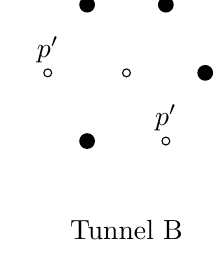
\begin{tikzpicture}

          \begin{scope}[xshift=2cm, yshift=2cm]
            \draw(0,0) circle [radius=0.05];
            \node[above] at (180:1) {$p^\prime$};
            \node[above] at (-60:1) {$p^\prime$};

            \foreach \theta in {-60,180}{
              \draw[transform canvas={shift=(\theta:1)}](0,0) circle [radius=0.05];
            }
            
            \foreach \theta in {0,60,120,-120}{
 	            \fill[transform canvas={shift=(\theta:1)}](0,0) circle [radius=0.1];
            }
          \end{scope}

          \node at (2,0) {Tunnel B};
        \end{tikzpicture}
      \end{minipage}

      \begin{minipage}{0.3\hsize}
        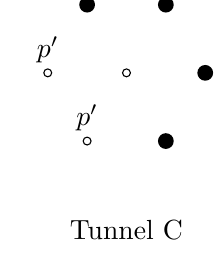
\begin{tikzpicture}

          \begin{scope}[xshift=2cm, yshift=2cm]
            \draw(0,0) circle [radius=0.05];
            \node[above] at (180:1) {$p^\prime$};
            \node[above] at (-120:1) {$p^\prime$};

            \foreach \theta in {-120,180}{
              \draw[transform canvas={shift=(\theta:1)}](0,0) circle [radius=0.05];
            }
            
            \foreach \theta in {0,60,-60,120}{
              \fill[transform canvas={shift=(\theta:1)}](0,0) circle [radius=0.1];
            }
          \end{scope}

          \node at (2,0) {Tunnel C};
        \end{tikzpicture}
      \end{minipage}
      
    \end{tabular}
    \caption{All possible tunnel sections: straight, obtuse turn, and acute turn}
    \label{TTT_tunnel}
  \end{center}
\end{figure}



%\begin{figure}
%  \begin{center}
%    \begin{tikzpicture}
%      \draw[thick, gray]
%      (0.5,1)--(0,1)--(0,4)--(4,4)--(4,1)--(3.5,1);
%      \node at(2,1) {Outside};
%      \node at (2,3.2) [rectangle, draw, rounded corners] (enter) {Entrance of a tunnel};
%      \node at(2,1.8) [rectangle, draw, rounded corners] (outside) {Otherwise};
%
%      
%      
%      \draw[thick, gray]
%      (7.5,1)--(7,1)--(7,4)--(11,4)--(11,1)--(10.5,1);
%      \node at(9,1) {Inside of a tunnel};
%      \node at(9,3.2) [rectangle, draw, rounded corners] (next-tunnel) {Successor in inside};
%      \node at(9,1.8) [rectangle, draw, rounded corners] (next-outside) {Successor in outside};
%
%      \draw[->]
%      (outside) edge [bend left, blue] node[left] {$s=b,\Delta=-1$} (enter)
%                   edge [loop left, blue] node[below left] {$s=b,\Delta=\pm 0$} (outside)
%      (enter)   edge [bend left, blue] node[above] {$s=b,\Delta=-1$} (next-tunnel)
%                edge [bend left, blue] node[above] {$s=b,\Delta=-a$} (next-outside)
%                edge [bend left, blue] node[right] {$s=b,\Delta=\pm 0$}  (outside)
%      (next-tunnel) edge[teal]         node[right] {$s=t,\Delta=-a$} (next-outside)
%                edge [loop right, teal]node[right] {$s=t,\Delta=\pm 0$}    (next-tunnel)
%      (next-outside) edge[bend left, teal] node[above] {$s=t,\Delta=+a$}  (outside)
%                edge [bend left, teal]     node[above] {$s=t,\Delta=+(a-1)$}(enter)
%      ;
%      
%    \end{tikzpicture}
%    \caption{Increment on Tunnel A,B}
%    \label{TTT_position}
%  \end{center}
%\end{figure}


%\begin{figure}
%  \begin{center}
%    \begin{tikzpicture}
%      \node at (0,4)   [rectangle, draw,rounded corners] (outside1) {Outside of tunnels};
%      \node at (3.5,4) [rectangle, draw,rounded corners] (enter1)   {Entrance of a tunnel};
%      \node at (7,4)   [rectangle, draw, rounded corners] (inside1) {Inside of a tunnel C};
%      \node at (11,4)  [rectangle, draw, rounded corners] (exit1)   {Inside of a tunnel A or B};
%      \draw[->] (outside1)--(enter1);
%      \draw[->] (enter1)  --(inside1);
%      \draw[->] (inside1) --(exit1);
%      
%      
%      \node at (0,3)   [rectangle, draw,rounded corners] (outside2) {Inside of a tunnel};
%      \node at (3.5,3) [rectangle, draw,rounded corners] (enter2)   {Entrance of a tunnel};
%      \node at (7,3)   [rectangle, draw, rounded corners] (inside2) {Inside of a tunnel C};
%      \node at (11,3)  [rectangle, draw, rounded corners] (exit2)   {Inside of a tunnel A or B};     
%      \draw[->] (outside2)--(enter2);
%      \draw[->] (enter2)  --(inside2);
%      \draw[->] (inside2) --(exit2);
%
%      \node at (0,1)   [rectangle, draw,rounded corners] (outside3) {Outside of tunnels};
%      \node at (3.5,1) [rectangle, draw,rounded corners] (enter3)   {Entrance of a tunnel};
%      \node at (7,1)   [rectangle, draw, rounded corners] (inside3) {Inside of a tunnel C};
%      \node at (11,1)  [rectangle, draw, rounded corners] (exit3)   {Outside of tunnels};     
%      \draw[->] (outside3)--(enter3);
%      \draw[->] (enter3)  --(inside3);
%      \draw[->] (inside3) --(exit3);
%
%      \node at (0,0)   [rectangle, draw,rounded corners] (outside4) {Inside of atunnel};
%      \node at (3.5,0) [rectangle, draw,rounded corners] (enter4)   {Entrance of a tunnel};
%      \node at (7,0)   [rectangle, draw, rounded corners] (inside4) {Inside of a tunnel C};
%      \node at (11,0)  [rectangle, draw, rounded corners] (exit4)   {Outside of tunnels};     
%      \draw[->] (outside4)--(enter4);
%      \draw[->] (enter4)  --(inside4);
%      \draw[->] (inside4) --(exit4);
%    \end{tikzpicture}
%    \caption{Case of Tunnel C}
%    \label{TTT_tunnelC_graph}
%  \end{center}
%\end{figure}






\begin{proof}[lemma \ref{TTT_neighbor_lemma}]
Any transcript bead has predecessor and successor except for the first and last beads. If the bead does not have any free hand, then it uses hands with $\alpha$ neighbors. Thus, lemma \ref{TTT_neighbor_lemma} is clearly true.
\end{proof}

\begin{proof}[lemma \ref{TTT_entrance_Tab}]
Fig.\ref{TTT_tunnel_direction} exhibits all the three kinds of entrance of tunnel A, B.
Let $w[i]$ be stabilized at an entrance point of Tunnel $A$ or $B$.
All cases are $\#bc(C_{i-1}) > \#bc(C_{i})$ as follows.


\begin{itemize}
\item{Case of $t_0$}\\
  Let us consider points $n_3,n_4$. At least one of the points $n_3$ or $n_4$ is free because if both of them are occupied, $p^\prime$ is inside of tunnel. If $n_3$ is free, then $p^\prime$ has to be bound to a bead other than $n_1$ to deterministically stabilize. In this situation, at least three neighbors of $n_1$ are free, that is, $n_1$ has at least one free hand from lemma \ref{TTT_neighbor_lemma}. Hence, $p^\prime$ must be bound to $n_1$. Thus, a case of $t_0$ consumes two hands and it does not supply any binding capabilities.

\item{Case of $t_{\pm 60}$}\\
  In this case, too, $n_4$ or $n_5$ is free. If $n_5$ is free, $p^\prime$ has to be bound to $n_1$ or $n_2$. If $n_5$ is occupied, then $n_4$ is free. This time, by $n_2$ has some free hands so $p^\prime$ has to be bound to $n_2$.
  

  In this situation, $p^\prime$ is able to supply a binding capabilities which could bind a bead into $n_4$ or $n_5$. However, $n_2$ and $n_3$ are part of a contiguous conformation. According to Jordan curve theorem, any successors of $p^\prime$ cannot reach a point $n_4$ or $n_5$ so this capability is inactive. Thus, in the case of $t_{\pm 60}$ $\#bc(C_{i-1}) > \#bc(C_{i})$.

\item{Case of $t_{\pm 120}$}\\
  Binding capabilities that $p^\prime$ supplies are inactive according to Jordan curve theorem on $n_1$ and $n_2$. Moreover, $p^\prime$ has to be bound to one of $n_3, n_4, n_5$ in order to deterministically stabilize.
Thus, in the case of $t_{\pm 120}$ is $\#bc(C_{i-1}) > \#bc(C_{i})$.
  
\end{itemize}

\begin{figure}
  \begin{center}
    \begin{tabular}{ccc}
    
    
      \begin{minipage}{0.3\hsize}
      \centering
        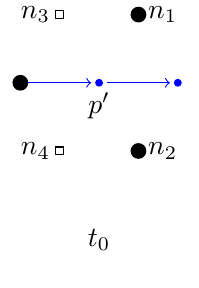
\begin{tikzpicture}
	 \draw[->,white] (120:0.8)--(120:0.1);%for adjustment
          
            \fill[blue] (0,0) circle [radius=0.05];
            \node[below] at (0,0) {$p^\prime$};

            \foreach \theta in {0}{
              \fill[transform canvas={shift=(\theta:1)},blue](0,0) circle [radius=0.05];
            }
            
            \foreach \theta in {60,-60,180}{
              \fill[transform canvas={shift=(\theta:1)}](0,0) circle [radius=0.1];
            }

            \foreach \theta in {120,-120}{
              \draw[transform canvas={shift=(\theta:1)}](-0.05,-0.05) rectangle (0.05,0.05);
            }
            
            \draw[->, blue] (180:0.9)--(180:0.1);
            \draw[->, blue] (0:0.1)--(0:0.9);

            \node[transform canvas={shift=(60:1)},right] {$n_1$};
            \node[transform canvas={shift=(-60:1)},right] {$n_2$};
            \node[transform canvas={shift=(120:1)},left] {$n_3$};
            \node[transform canvas={shift=(-120:1)},left] {$n_4$};


          \node at (0,-2) {$t_{0}$};
        \end{tikzpicture}
      \end{minipage}

      

      \begin{minipage}{0.3\hsize}
      \centering
        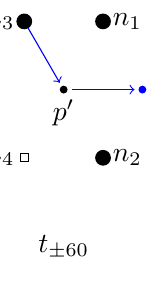
\begin{tikzpicture}

            \fill(0,0) circle [radius=0.05];
            \node[below] at (0,0) {$p^\prime$};

            \foreach \theta in {0}{
              \fill[transform canvas={shift=(\theta:1)},blue](0,0) circle [radius=0.05];
            }
            
            \foreach \theta in {60,-60,120}{
              \fill[transform canvas={shift=(\theta:1)}](0,0) circle [radius=0.1];
            }

            \foreach \theta in {180,-120}{
              \draw[transform canvas={shift=(\theta:1)}](-0.05,-0.05) rectangle (0.05,0.05);
            }
            
            \draw[->, blue] (120:0.9)--(120:0.1);
            \draw[->, blue] (0:0.1)--(0:0.9);

            \node[transform canvas={shift=(60:1)},right] {$n_1$};
            \node[transform canvas={shift=(-60:1)},right] {$n_2$};
            \node[transform canvas={shift=(120:1)},left] {$n_3$};
            \node[transform canvas={shift=(-120:1)},left] {$n_4$};
            \node[transform canvas={shift=(180:1)},left] {$n_5$};

          \node at (0,-2) {$t_{\pm 60}$};
        \end{tikzpicture}
      \end{minipage}

      \begin{minipage}{0.3\hsize}
      \centering
        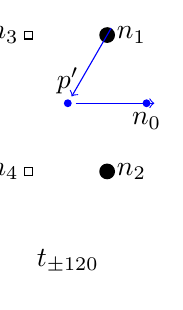
\begin{tikzpicture}
            \fill[blue](0,0) circle [radius=0.05];
            \node[above] at (0,0) {$p^\prime$};

            \foreach \theta in {0}{
              \fill[transform canvas={shift=(\theta:1)}, blue](0,0) circle [radius=0.05];
            }
            
            \foreach \theta in {60,-60}{
              \fill[transform canvas={shift=(\theta:1)}](0,0) circle [radius=0.1];
            }

            \foreach \theta in {180,-120,120}{
              \draw[transform canvas={shift=(\theta:1)}](-0.05,-0.05) rectangle (0.05,0.05);
            }
            
            \draw[->, blue] (60:1.1)--(60:0.1);
            \draw[->, blue] (0:0.1)--(0:1.1);

            \node[transform canvas={shift=(0:1)},below] {$n_0$};
            \node[transform canvas={shift=(60:1)},right] {$n_1$};
            \node[transform canvas={shift=(-60:1)},right] {$n_2$};
            \node[transform canvas={shift=(120:1)},left] {$n_3$};
            \node[transform canvas={shift=(-120:1)},left] {$n_4$};
            \node[transform canvas={shift=(180:1)},left] {$n_5$};

          \node at (0,-2) {$t_{\pm 120}$};
        \end{tikzpicture}
      \end{minipage}
      
    \end{tabular}
    \caption{Direction into a entrance}
    \label{TTT_tunnel_direction}
  \end{center}
\end{figure}

\end{proof}

\begin{proof}[lemma \ref{TTT_exit}]
Fig.\ref{TTT_tunnel_exit} exhibits all the two kinds of exit of tunnel. 
At least one of points $n_1$ or $n_2$ is free because if both of them are occupied, $p^\prime$ is inside of tunnel.

\begin{paragraph}{}
$\delta = 1, \alpha = 2$\\
Let $\Xi$ be a unary oritatami system at $\delta = 1, \alpha = 2$. We assume $S[h..i+1] = bt^{(i-h)}b \quad (h<i)$ and
let $a$ be $\#bc(C_{i-2}) - \#bc(C_{i-1}) = a$. Then, $\#bc(C_{i}) - \#bc(C_{i-1}) \leq a$ as follows. Also, if $i - h > 1$ and $j$ is such that $h<j<i$, then $\#bc(C_{j-1}) \geq \#bc(C_{j})$ because all neighbors of $w[j]$ are occupied by beads forming the tunnel so that any $w[i+1..]$ cannot reach neighbors of $w[j]$. Thus, $\#bc(C_{h-1}) \geq \#bc(C_i)$ and $\#bc(C_{i-2}) \geq \#bc(C_i)$.
\end{paragraph}

\begin{itemize}
\item{Case of both $n_1$ and $n_2$ being free}\\
  This case can be regarded the same as entrance. See Fig.\ref{TTT_tunnel_exit} (Left). Predecessor $n_5$ has to be bound to $n_4$ and $n_5$ because both of $n_3$ and $n_4$ have binding capabilities. Hence, $a \geq 2$. This time, $\alpha = 2$, that is, this case $\#bc(C_{i}) - \#bc(C_{i-1}) \leq a$.
  
\item{Case of $n_1$ is occupied}\\
  See Fig.\ref{TTT_tunnel_exit} (Right). If $n_1$ is occupied, then $n_2$ is free so that $n_5$ has to be bound $n_4$. Hence,  $a \geq 1$. This case can supply two binding capabilities but $p^\prime$ can bind to only one of $n_0$ or $n_2$ because $n_0$ or $n_2$ will be occupied by the successor of $p^\prime$. Therefore, this case $\#bc(C_{i}) - \#bc(C_{i-1}) \leq a$.
  
\end{itemize}

\begin{paragraph}{}
$\delta = 1, \alpha \geq 3$\\
Let $\Xi$ be a unary oritatami system at $\delta = 1, \alpha \geq 3$. We assume $w[i]$ is stabilized at exit of tunnel.
In all cases $\#bc(C_{i-1}) > \#bc(C_{i})$. Moreover, if $S[k] = t (k \leq i)$, then $\#bc(C_{k-1}) > \#bc(C_{k})$ because both sides of the path $p$ in Fig.\ref{TTT_inside_tunnel} ($n_1, n_2$) have two free points and one of $n_1, n_2$ is not the predecessor so that it has hand and moreover that $w[k]$ supplies any binding capabilities because its neighbors are occupied by beads of tunnel.
\end{paragraph}

\begin{itemize}
\item{Case of $n_1$ and $n_2$ are free}\\
  In $\alpha \geq 3$, if three neighbors of a bead leave, then it can supply two binding capabilities. Therefore predecessor $n_5$ has to be bound $n_3$ and $n_4$, and $p^\prime$, too. In this case, at least four bindings are consumed and at most two are added. Thus, it consumes some binding capabilities, overall.
  
\item{Case of $n_1$ is occupied}\\
  In this case, $n_4$ leave at least two bindings and $n_3$, $n_1$ also leave at least one binding. Therefore $n_5$ has to be bound $n_3$ and $n_4$, and $p^\prime$ also has to be bound $n_1$ and $n_4$. In this case, at least four bindings are consumed and at most two are added. Thus, it consumes some binding capabilities, totally.
\end{itemize}


\begin{figure}
  \centering
    \begin{tabular}{cc}
    \begin{minipage}{0.66\hsize}
    \centering
      \begin{tabular}{cc}
      \begin{minipage}{0.45\linewidth}
      \centering
        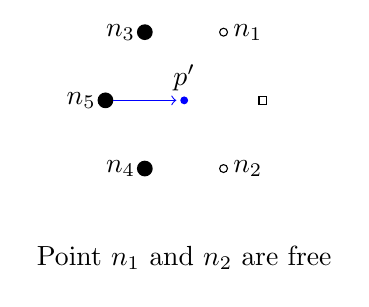
\begin{tikzpicture}
	\draw[white] (0:0) -- (120:1);
	\draw[white] (0:0) -- (-60:1);
	\draw[white] (0:0) -- (0:1);

            \fill[blue](0,0) circle [radius=0.05];
            \node[above] at (0,0) {$p^\prime$};

            
            \foreach \theta in {120,-120,180}{
              \fill[transform canvas={shift=(\theta:1)}](0,0) circle [radius=0.1];
            }

            \foreach \theta in {0}{
              \draw[transform canvas={shift=(\theta:1)}](-0.05,-0.05) rectangle (0.05,0.05);
            }
            \draw (-60:1) circle [radius=0.05];
            \draw (60:1) circle [radius=0.05];

            \draw[->, blue] (180:0.9)--(180:0.1);



            \node[transform canvas={shift=(60:1)},right] {$n_1$};
            \node[transform canvas={shift=(-60:1)},right] {$n_2$};
            \node[transform canvas={shift=(120:1)},left] {$n_3$};
            \node[transform canvas={shift=(-120:1)},left] {$n_4$};
            \node[transform canvas={shift=(180:1)},left] {$n_5$};

          \node at (0,-2) {Point $n_1$ and $n_2$ are free};
        \end{tikzpicture}
      \end{minipage}

      \begin{minipage}{0.45\linewidth}
      \centering
        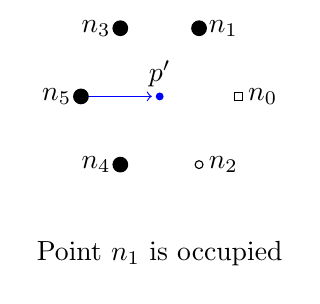
\begin{tikzpicture}
	\draw[white] (0:0) -- (0:1);
	\draw[white] (0:0) -- (120:1);
	\draw[white] (0:0) -- (-90:2);

            \fill[blue](0,0) circle [radius=0.05];
            \node[above] at (0,0) {$p^\prime$};
            
            \foreach \theta in {120,-120,180,60}{
              \fill[transform canvas={shift=(\theta:1)}](0,0) circle [radius=0.1];
            }

            \foreach \theta in {0}{
              \draw[transform canvas={shift=(\theta:1)}](-0.05,-0.05) rectangle (0.05,0.05);
            }
            \draw (-60:1) circle [radius=0.05];

            \draw[->, blue] (180:0.9)--(180:0.1);

            \node[transform canvas={shift=(0:1)},right] {$n_0$};
            \node[transform canvas={shift=(60:1)},right] {$n_1$};
            \node[transform canvas={shift=(-60:1)},right] {$n_2$};
            \node[transform canvas={shift=(120:1)},left] {$n_3$};
            \node[transform canvas={shift=(-120:1)},left] {$n_4$};
            \node[transform canvas={shift=(180:1)},left] {$n_5$};


          
          \node at (0,-2) {Point $n_1$ is occupied};
        \end{tikzpicture}
      \end{minipage}
    \end{tabular}
    \caption{Exit of Tunnel}
    \label{TTT_tunnel_exit}
    \end{minipage}
    
    \begin{minipage}{0.33\hsize}
    \centering
     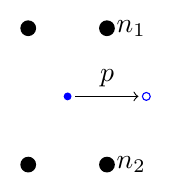
\begin{tikzpicture}
	\draw[white] (0:0) -- (120:1);
	\draw[white] (0:0) -- (-60:1);
            \fill[blue](0,0) circle [radius=0.05];
            \draw[blue] (0:1) circle [radius = 0.05];
            \draw[->] (0:0.1) -- node[above]{$p$} (0:0.9);
            
            \foreach \theta in {60, -60, 120,-120,180}{
              \fill[transform canvas={shift=(\theta:1)}](0,0) circle [radius=0.1];
            }
            \node[transform canvas={shift=(60:1)},right] {$n_1$};
            \node[transform canvas={shift=(-60:1)},right] {$n_2$};
                \end{tikzpicture}
                
    \caption{Inside tunnel}
    \label{TTT_inside_tunnel}
    \end{minipage}
 
    \end{tabular}
\end{figure}
\end{proof}

\begin{proof}[lemma \ref{TTT_tunnelC_lemma}]
Let $\Xi$ be a unary oritatami system at $\delta = 1, \alpha = 2$.
Assume $S[h..i+1] = bt^{i-h}b (h<i)$. If at least one of $w[h+1..i]$ are stabilized by tunnel $C$, then only $w[h+1]$ can use tunnel $C$ because if $w[g]$ which is one of $w[h+2..i]$, with $h+2 \leq g \leq i$ is stabilized by tunnel $C$, $C_g$ is a terminal.


Let us consider stabilization $S[h-1..h+1] = tbt$ or $S[h-1..h+1] = bbt$ as follows. In result, $\#bc(C_{h-3}) > \#bc(C_{h+1})$. In addition according to lemma\ref{TTT_exit} $\#bc(C_{h+1}) \geq \#bc(C_{i})$. Thus, $\#bc(C_{h-3}) > \#bc(C_{h+1})$ and $\#bc(C_{h-3}) > \#bc(C_{i})$.
\\

\subsubsection{Case of $S[h-1..h+1] = tbt$}
Fig.\ref{TTT_tunnelC_enter_usingTunnel} exhibits all the two kinds of stabilization depending on structures of tunnel C.

\begin{itemize}
\item{Left of Fig.\ref{TTT_tunnelC_enter_usingTunnel}}\\
  In this figure, Bead $n_4$ has at least one binding so that $w[h-1]$ has to bound $n_4$. Moreover, $w[h]$ has to bind to one of $n_1, n_2, n_3$ in order to stabilize deterministically. On the other hand, $w[h+1]$ can supply two bindings but has only two free neighbors. One of them is occupied by a successor. Therefore $w[h+1]$ can only bind one of $n_5, n_6$, that is, $w[h+1]$ supplies at most one binding. Thus, this case $\#bc(C_{h-1}) > \#bc(C_{h+1})$.

\item{Right of Fig.\ref{TTT_tunnelC_enter_usingTunnel}}\\
  These cases are divided on number of capabilities that $w[h-1]$ consumes.
  \begin{itemize}
  \item[-]{$w[h-1]$ does not consume any bindings}\\
  According to lemma\ref{TTT_exit}, $\#bc(C_{h-3}) \geq \#bc(C_{h-1})$ because of $S[h-1] = t$.
    $w[h]$ has to bound one of $n_1, n_2, n_3$ in order to stabilize deterministically so that  $\#bc(C_{h-1}) > \#bc(C_{h})$.
    $w[h+1]$ has to be bound to $w[h-1]$ because $w[h-1]$ has bindings, that is, $w[h+1]$ consumes at least one hand and supplies at most one hand so that $\#bc(C_{h}) \geq \#bc(C_{h+1})$. Thus, in this cases $\#bc(C_{h-3}) > \#bc(C_{h+1})$.
%     This time, let us consider either $n_4$ is occupied or not. If $n_4$ is occupied, then $w[h-1]$ has no active bindings that is this situation consumes some binding capabilities. If $n_4$ is free and $w[h+2]$ is stabilized in $n_4$, then $w[h-1]$ has to bind $w[h+2]$. Therefore, In this case, stabilization of $w[h-1..h+2]$ consumes some bindings. If $n_4$ is free and $w[h+2]$ is stabilized except $n_4$, then this oritatami system has to use two binding capabilities in order to bind $w[h+2]$. Therefore, in this case consumes some bindings. Thus in this cases $\#bc(C_{h-1}) > \#bc(C_{h+2})$.

  \item[-]{$w[h-1]$ consumes one binding}\\
    In this case, $w_{h}$ has to be bound one of $n_1, n_2, n_3$. In addition, $w[h-1]$ and $w[h+1]$ are not supply any bindings. Thus, in this cases consume some binding capabilities.
  \item[-]{$w[h-1]$ consumes two bindings}\\
    In this case, $w[h-1]$ already consumes two binding. $w[h]$ has to be bound. $w[h+1]$ supplies two bindings. Thus, in this cases $\#bc(C_{h-1}) > \#bc(C_{h+1})$.
   
  \end{itemize}
\end{itemize}
\begin{figure}
  \centering
    \begin{tabular}{cc}
      
      \begin{minipage}{0.48\hsize}
      \centering
        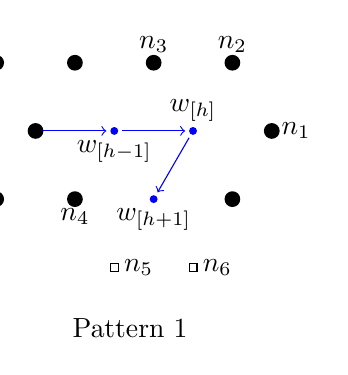
\begin{tikzpicture}

          \fill[transform canvas={shift=(0:0)}](0,0) circle [radius=0.1];
          
          \foreach \theta in {60,-60,120,-120,180}{
            \fill[transform canvas={shift=(\theta:1)}](0,0) circle [radius=0.1];
          }

          \fill[blue](0:1) circle [radius=0.05];
          \draw[->, blue] (0:0.1)--(0:0.9);

          \node[below] at (-60:1) {$n_4$};

          \begin{scope}[shift=(0:2)]
            \fill[blue](0,0) circle [radius=0.05];

            
            \foreach \theta in {120,60,-60,0}{
             \fill[transform canvas={shift=(\theta:1)}](0,0) circle [radius=0.1];
            }

            \draw[->, blue] (180:0.9)--(180:0.1);
            \draw[->, blue] (-120:0.1)--(-120:0.9);

            \node[below] at (180:1) {$w_{[h-1]}$};
            \node[above] at (0:0) {$w_{[h]}$};
            \node[below] at (-120:1) {$w_{[h+1]}$};

            \node[above] at (120:1) {$n_3$};
            \node[above] at (60:1) {$n_2$};
            \node[right] at (0:1) {$n_1$};

            \begin{scope}[shift=(-120:1)]
              \fill[blue](0,0) circle [radius=0.05];
              \foreach \theta in {-120,-60}{
                \draw[transform canvas={shift=(\theta:1)}](-0.05,-0.05) rectangle (0.05,0.05);
              }

              \node[right] at (-120:1) {$n_5$};
              \node[right] at (-60:1) {$n_6$};
            \end{scope}
            
          \end{scope}

          \node at (1.2,-2.5) {Pattern 1};
        \end{tikzpicture}
      \end{minipage}

      \begin{minipage}{0.48\hsize}
      \centering
        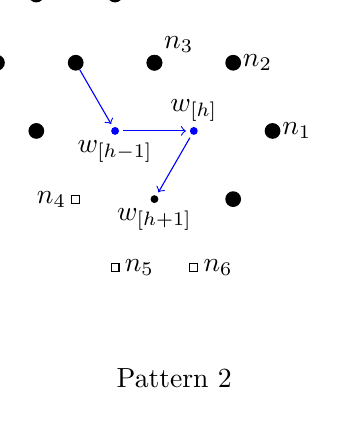
\begin{tikzpicture}

          \fill(0,0) circle [radius=0.1];
          
          \foreach \theta in {60,0,120,-120,180}{
            \fill[transform canvas={shift=(\theta:1)}](0,0) circle [radius=0.1];
          }

          \draw[->, blue] (-60:0.1)--(-60:0.9);


          \begin{scope}[shift=(-60:1),shift=(0:1)]
            \fill[blue](0,0) circle [radius=0.05];
            \fill[blue](180:1) circle [radius=0.05];

            
            \foreach \theta in {120,60,0,-60}{
              \fill[transform canvas={shift=(\theta:1)}](0,0) circle [radius=0.1];
            }

            \draw[->, blue] (180:0.9)--(180:0.1);
            \draw[->, blue] (-120:0.1)--(-120:0.9);

            \node[below] at (180:1) {$w_{[h-1]}$};
            \node[above] at (0:0) {$w_{[h]}$};
            \node[below] at (-120:1) {$w_{[h+1]}$};

            \node[above right] at (120:1) {$n_3$};
            \node[right] at (60:1) {$n_2$};
            \node[right] at (0:1) {$n_1$};

            \begin{scope}[shift=(-120:1)]
              \fill(0,0) circle [radius=0.05];
              \foreach \theta in {180,-120,-60}{
                \draw[transform canvas={shift=(\theta:1)}](-0.05,-0.05) rectangle (0.05,0.05);
              }

              \node[left] at (180:1) {$n_4$};
              \node[right] at (-120:1) {$n_5$};
              \node[right] at (-60:1) {$n_6$};
            \end{scope}
            
          \end{scope}

          \node at (1.25,-4) {Pattern 2};
        \end{tikzpicture}
      \end{minipage}

      
      
    \end{tabular}
    \caption{Case of $S[h-1..h+1] = tbt$}
    \label{TTT_tunnelC_enter_usingTunnel}
\end{figure}


\subsubsection{Case of $S[h-1..h+1] = bbt$}
Let us consider number of consumed bindings by $w[h-1]$ (Fig.\ref{TTT_tunnelC_enter_usingBond}).

\begin{itemize}
\item{$w[h-1]$ consumes one binding}\\
  In this situation, $w[h-1]$ supplies one active binding whereas $w[h+1]$ consumes this binding. In addition, $w[h]$ has to bound to one of $n_1, n_2, n_3$.
  Thus, in this cases consume some binding capabilities.

\item{$w[h-1]$ consumes two bindings}\\
  In this case, $w[h-1]$ already consumes two binding. $w[h]$ has to be bound. $w[h+1]$ supplies at most two bindings. Thus, in this cases consume some binding capabilities.
\end{itemize}



\begin{figure}
  \begin{center}
        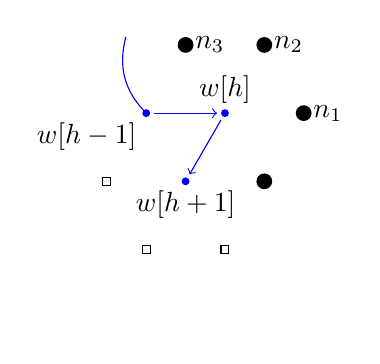
\begin{tikzpicture}
        \draw[->,white] (-70:0.1) -- (-70:3);
          \foreach \theta in {60,-60,120,0}{
            \fill[transform canvas={shift=(\theta:1)}](0,0) circle [radius=0.1];
          }

          \fill[blue](180:1) circle [radius=0.05];
          \fill[blue](0:0) circle [radius=0.05];

          \draw[transform canvas={shift=(180:1)}, blue] (105:1) edge[bend right] (105:0);
          \draw[->, blue] (180:0.9) -- (180:0.1);
          \draw[->, blue] (-120:0.1) -- (-120:0.9);

          \node[below left] at (180:1) {$w[h-1]$};
          \node[above] at (0:0) {$w[h]$};
          \node[below] at (-120:1) {$w[h+1]$};

          \node[right] at (120:1) {$n_3$};
          \node[right] at (60:1) {$n_2$};
          \node[right] at (0:1) {$n_1$};

          \begin{scope}[shift=(-120:1)]
            \fill[blue](0,0) circle [radius=0.05];
            \foreach \theta in {-120,-60,180}{
              \draw[transform canvas={shift=(\theta:1)}](-0.05,-0.05) rectangle (0.05,0.05);
            }
            
          \end{scope}
        \end{tikzpicture}
    \caption{Case of $S[h-1..h+1] = bbt$}
    \label{TTT_tunnelC_enter_usingBond}
  \end{center}
\end{figure}

\end{proof}




%%%%%%%%%%%%%%%%%%%%%%%%%%%%%%%%%%%%%%%%%%%%%%%%%%%%%%%%%
%/////////////////////////////////////////////////
%%%%%%%%%%%%%%%%%%%%%%%%%%%%%%%%%%%%%%%%%%%%%%%%%%%%%%%%%


\subsection{On structures provided by a unary and $\delta = 1$ oritatami system}
\begin{theorem}[$\delta= 1, \alpha=2$]
Let $\Xi$ be a unary oritatami system of $\delta = 1, \alpha = 2$. It can yield infinite structures but they are only zig-zag conformation.
\end{theorem}

\begin{proof}
By Tunnel Troll Theorem, any tunnel sections which represented in $bbt^+$ or $bt^+bt^+$ consume binding capabilities. If the sequence $S$ is free from any subsequence of the form $bt^+bt^+$, then it can factorize as $S = u_1 u_2 u_3 \cdots$ for some $u_1 , u_2 , u_3 , \cdots \in \{b\} \cup bbt^+$. Assume the length of $\sigma$ is $n$, seed supplies at most $2n$ binding capabilities. Therefore formula \ref{TTT_only_bond} hold.

\begin{eqnarray}
  \exists i \in \mathbb{N} \quad s.t. \quad u_{i-1} , u_i , u_{i+1} , u_{i+2} , \cdots \in \{ b \}
  \label{TTT_only_bond}
\end{eqnarray}


Let us represent $S$ as $S[i.i+1...] = v_i v_{i+1} v_{i+2} \cdots$ for some $v_i, v_{i+1}, v_{i+2}, \cdots \in \{ a, o\}$ where if $v_k$ is $a$, then $v_{k+1}$ is bound to $v_{k-1}$, if $v_k$ is $o$, then $v_{k+1}$ is NOT bound to $v_{k-1}$.


Let us consider the case of $v_k$ is $o$. See Fig.\ref{TTT_case_of_o}. $w[i-1]$ consumes some binding capabilities because $v_{i-1}$ is $b$. If the number of $w[i-1]$'s bindings is one binding, then $w[i+1]$ has to be bound except $n_1$ or $n_2$ so that $w[i+1]$ must consumes two bindings except the case of $n_1$ and $n_2$ are occupied and $w[i]$ consumes at least one binding. If $n_1$ and $n_2$ are occupied, then $w[i-1]$'s bindings are inactive, that is, $w[i-1]$ consumes two binding capabilities. Therefore, this case consumes binding capabilities. If $w[i-1]$ dose Not have any bindings, then $w[i-1]$ already consumes two bindings. In addition, $w[i]$ and $w[i+1]$ consume at least one binding. Therefore this case consumes binding capabilities. Thus, the formula \ref{TTT_only_a} hold and according to the formula \ref{TTT_only_bond} and the formula \ref{TTT_only_a}, the formula \ref{TTT_structure} is hold. Thus, in this case, oritatami system can yield infinite structures but they are only zig-zag conformation.

\end{proof}

\begin{eqnarray}
  \exists j \in \mathbb{N} \quad s.t. \quad u_j , u_{j+1} , u_{j+2} , \cdots \in \{ a \}
  \label{TTT_only_a}
\end{eqnarray}

\begin{eqnarray}
  | S | > \forall m \in \mathbb{N} \quad \to \quad \exists n \in \mathbb{N} \quad s.t. \quad S[n], S[n+1], \cdots \in \{ a \}
  \label{TTT_structure}
\end{eqnarray}

\begin{figure}
  \begin{center}
    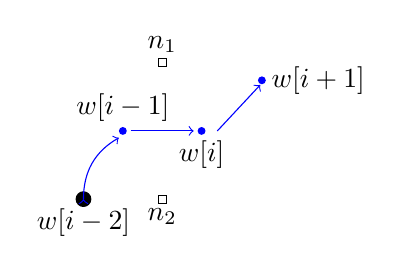
\begin{tikzpicture}
      
      \fill[transform canvas={shift=(-120:1)}](0,0) circle [radius=0.1];
      
      \fill[blue](0:0) circle [radius=0.05];
      \fill[blue](0:1) circle [radius=0.05];
      \fill[shift=(0:1), blue](40:1) circle [radius=0.05];

      \draw[->, blue] (-120:1) edge[bend left] (-120:0.1);
      \draw[->, blue] (0:0.1) -- (0:0.9);
      \draw[->,transform canvas={shift=(0:1.2)}, blue] (50:0) -- (47:0.8);
      
      \draw[shift=(60:1)](-0.05,-0.05) rectangle (0.05,0.05);
      \draw[shift=(-60:1)](-0.05,-0.05) rectangle (0.05,0.05);
      
      \node[below] at (-120:1) {$w[i-2]$};
      \node[above] at (0:0) {$w[i-1]$};
      \node[below] at (0:1) {$w[i]$};
      \node[right, shift=(0:1)] at (40:1) {$w[i+1]$};

      \node[above] at (60:1) {$n_1$};
      \node[below] at (-60:1) {$n_2$};
        
    \end{tikzpicture}
    \caption{Case of $S[i]$}
    \label{TTT_case_of_o}
  \end{center}
\end{figure}

\begin{theorem}[$\delta = 1, \alpha = 3$]
Let $\Xi$ be a unary oritatami system of $\delta = 1, \alpha = 3$. It can yield only finite structures whose size is $\mathcal{O}(n)$.
\end{theorem}

\begin{lemma}
\label{TTT_a3_2b_lemma}
 Let $p$ be a point whose neighbors is occupied at least two point. If $w[i]$ is not stabilized and $w[i-1]$ includes neighbors of $p$, then $w[i]$ is stabilized at $p$ with at least one bond, $w[i]$ is stabilized at another point of $p$ otherwise with at least two bond except any neighbors of $p$ is occupied.
\end{lemma}

\begin{proof}[proof of lemma]
Assume the transcript is stabilized until $w[i-1]$. One of neighbors of $p$ is not $w[i-1]$ where this bead regards $n_1$. If $w[i-1]$ include neighbors of $p$ and $w[i]$ is stabilized at another point of $p$ with one bond. Then, any neighbors do not have bond without $w[i-1]$. Neighbors of $n_1$ have to be occupied at least five according to lemma \ref{TTT_neighbor_lemma} and two of them include neighbors of $p$ where each of them regards $n_2, n_3$. In the same way, five neighbors of $n_2$ and $n_3$ are occupied and each of one of them includes neighbors of $p$ where they regard $n_4, n_5$. one of $n_5$'s neighbors includes neighbors of $p$ where it regards $n_6$. Then, any neighbors of $p$ are occupied. That is, if some neighbors of $p$ are free, then there exists a bead which has bonds in neighbors.
\end{proof}

\begin{proof}
Let us show that $\#bc(C_{i-1}) > \#bc(C_i)$, that is, when $w[i]$ is stabilized, $w[i]$ uses at least two hands.
Let us assume $w[i]$ is able to be stabilized with using one hand. Fig.\ref{TTT_a3_w} exhibits all the three kinds of possibility of stabilized $w[i]$. Then, $w[i]$ can be also stabilized at $n_3$. 

\begin{paragraph}{Case of straight}
\begin{itemize}
\item[-] Case of $n_3$ is free\\
According to assumption, $w[i]$ uses only one hand. Therefore, any neighbors of $n_3$ are occupied according to the lemma\ref{TTT_a3_2b_lemma}. $n_3$ and the point which is stabilized $w[i]$ are free so that $n_1$ has some bond by lemma\ref{TTT_neighbor_lemma}. Accordingly, this situation is non-deterministic. Thus, $n_3$ and $n_4$ have to be occupied because of symmetry.

\item[-] Otherwise\\
Because of  $S[i] = b$, at least one of $n_1$ and $n_2$ have to be free. Let us regard that $n_1$ is free. Neighbors of $n_1$ have to be occupied and at least two neighbors of $n_{-1}$ have to be free for $n_1$ and $w[i]$. According to lemma\ref{TTT_neighbor_lemma}, $n_{-1}$ have some hand. Therefore $w[i]$ can be also stabilized $n_1$, that is, this situation is non-deterministic. Thus, one of $n_3$ and $n_4$ has to be free.
\end{itemize}

Therefore, this case is false.
\end{paragraph}

\begin{paragraph}{Case of obtuse}
\begin{itemize}
\item[-] Case of $n_3$ is free\\
Any neighbors of $n_3$ have to be occupied but the point which is stabilized $w[i]$ is free. Thus $n_3$ has to be occupied.
\item[-] Case of $n_4$ is free\\
According to lemma\ref{TTT_a3_2b_lemma}, $n_2$ has to be occupied because $n_4$ is free. Also $n_0$ has to be occupied from lemma\ref{TTT_neighbor_lemma}. Thus, only one of $n_0, n_3$ leave some hands or both of them do not leave any hands because $w[i]$ use only one bond.\\
If $n_0$ has some hands, then $n_3$ does not have any hands so that $n_{-3}$ is occupied. Also $n_{-3}$ must not have any hands so that $n_{-2}$ is occupied and also $n_{-1}$ is occupied. Therefore any neighbors of $w[i]$ are occupied so that $w[i+1]$ cannot provide.\\
If $n_3$ has some hands, then $n_0$ does not have any hands so that $n_{-1}$ is occupied. In the same previous way, any $n_{-2}, n_{-3}$ are occupied.  Therefore any neighbors of $w[i]$ are occupied.\\
If both of $n_0, n_3$ do not have any hands, then both of $n_{-1}, n_{-3}$ are occupied. If one of $n_{-1}, n_{-3}$ has some hands, the other does not have any hands so that $n_{-2}$ is occupied. If both of $n_{-1}, n_{-3}$ do not have any hands, $n_{-2}$ has to be occupied and $n_{-2}$ has some hands.Therefore any neighbors of $w[i]$ are occupied so that $w[i+1]$ cannot provide.\\
Thus $n_3$ has to be occupied in order to yield infinite structures.
\item[-] Case of $n_2$ is free\\
Any neighbors of $n_2$ have to be occupied so that $n_0$ is occupied. Any neighbors of $n_0$ except $n_2$ have to be also occupied but the point which is stabilized $w[i]$ is free. Thus $n_2$ has to be occupied.
\item[-] Case of $n_0$ is free\\
Any neighbors of $n_0$ have to be occupied so that $n_{-1}$ is occupied. Any neighbors of $n_{-1}$ except $n_0$ have to be also occupied but the point which is stabilized $w[i]$ is free. Thus $n_0$ has to be occupied. 
\end{itemize}

Therefore, any situations contradict $S[i] = b$.

\end{paragraph}



\begin{paragraph}{Case of acute}
\begin{itemize}
\item[-] Case of $n_4$ is free\\
$n_4$ and a point which is stabilized $w[i]$ are free so that  $w[i-2]$ has some hands according to lemma\ref{TTT_neighbor_lemma}.
However, $w[i]$ can be also stabilized $n_4$ in this case. Thus, $n_4$ has to be occupied.
\item[-] Case of $n_2$ is free\\
According to lemma\ref{TTT_a3_2b_lemma}, $n_0$ has to be occupied. $n_1$ has to be also occupied because of lemma\ref{TTT_neighbor_lemma}.
We consider this case just like case of obtuse and that $n_4$ is free. Then if $w[i-2]$ binds $w[i]$, any $n_{-1}, n_{-2}, n_{-3}$ are occupied. If $n_1$ binds $w[i]$, this case is same. Also if $n_1$ and $w[i-2]$ do not have any hand, any $n_{-1}, n_{-2}, n_{-3}$ are occupied. Therefore, $w[i+1]$ cannot be provided.
\item[-] Case of $n_0$ is free\\
Any neighbors of $n_0$ have to be occupied so that $n_{1}$ is occupied. Any neighbors of $n_{1}$ except $n_0$ have to be also occupied but the point which is stabilized $w[i]$ is free. Thus $n_0$ has to be occupied. 
\item[-] Case of $n_1$ is free\\
Any neighbors of $n_1$ have to be occupied so that $n_{-1}$ is occupied. Any neighbors of $n_{-1}$ except $n_1$ have to be also occupied but the point which is stabilized $w[i]$ is free. Thus $n_1$ has to be occupied. 
\end{itemize}

Therefore, any situations contradict $S[i] = b$.
\end{paragraph}\\


Hence, assumption that w[i] is able to be stabilized with using one hand is false.
Therefore, when w[i] is stabilized, w[i] uses at least two hands.
\end{proof}

\begin{figure}
  \begin{center}
  \begin{tabular}{c c c}
 \begin{minipage}{0.3\hsize}
 \centering
    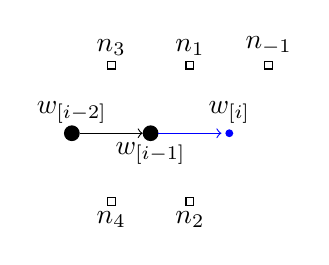
\begin{tikzpicture}
      
      \fill[shift=(180:1)] (0,0) circle [radius=0.1];
      \fill[shift=(180:0)] (0,0) circle [radius=0.1];
      
      \fill[blue](0:1) circle [radius=0.05];
      
      \draw[->] (180:0.9) -- (180:0.1);
      \draw[->, blue] (0:0.1) -- (0:0.9);

	\node[above] at (180:1) {$w_{[i-2]}$};
	\node[below] at (180:0) {$w_{[i-1]}$};
	\node[above] at (0:1) {$w_{[i]}$};

	\foreach \theta in {60,-60,120,-120}{
   	   \draw [shift=(\theta:1)] (-0.05,-0.05) rectangle (0.05,0.05);
  	}
	 \draw [shift=(60:1)] (0.95,-0.05) rectangle (1.05,0.05);
 	\node[above] at (60:1) {$n_1$};
	\node[below] at (-60:1) {$n_2$};
	\node[above] at (120:1) {$n_3$};
	\node[below] at (-120:1) {$n_4$};
	\node[above, shift=(0:1)] at (60:1) {$n_{-1}$};
    \end{tikzpicture}
    \end{minipage}
    
    \begin{minipage}{0.3\hsize}
    \centering
     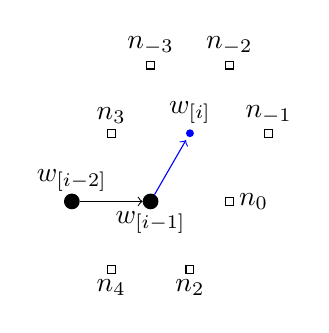
\begin{tikzpicture}
      
      \fill[shift=(180:1)] (0,0) circle [radius=0.1];
      \fill[shift=(180:0)] (0,0) circle [radius=0.1];
      
      \fill[blue](60:1) circle [radius=0.05];
      
      \draw[->] (180:0.9) -- (180:0.1);
      \draw[->, blue] (60:0.1) -- (60:0.9);

	\node[above] at (180:1) {$w_{[i-2]}$};
	\node[below] at (180:0) {$w_{[i-1]}$};
	\node[above] at (60:1) {$w_{[i]}$};


	\foreach \theta in {0,-60,120,-120}{
   	   \draw [shift=(\theta:1)] (-0.05,-0.05) rectangle (0.05,0.05);
  	}
	\draw [shift=(60:1)] (0.95,-0.05) rectangle (1.05,0.05);
	\draw [shift=(60:1), shift=(60:1)] (-0.05,-0.05) rectangle (0.05,0.05);
	\draw [shift=(60:1), shift=(120:1)] (-0.05,-0.05) rectangle (0.05,0.05);
	
 	\node[right] at (0:1) {$n_0$};
	\node[below] at (-60:1) {$n_2$};
	\node[above] at (120:1) {$n_3$};
	\node[below] at (-120:1) {$n_4$};
	\node[above, shift=(0:1)] at (60:1) {$n_{-1}$};
	\node[above, shift=(60:1)] at (60:1) {$n_{-2}$};
	\node[above, shift=(60:1)] at (120:1) {$n_{-3}$};
    \end{tikzpicture}
    \end{minipage}
    
    \begin{minipage}{0.3\hsize}
        \centering
     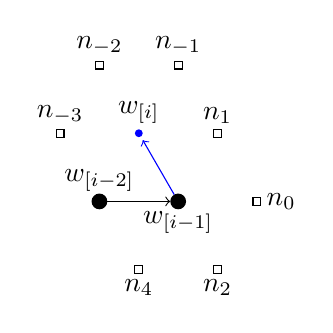
\begin{tikzpicture}
      
      \fill[shift=(180:1)] (0,0) circle [radius=0.1];
      \fill[shift=(180:0)] (0,0) circle [radius=0.1];
      
      \fill[blue](120:1) circle [radius=0.05];
      
      \draw[->] (180:0.9) -- (180:0.1);
      \draw[->, blue] (120:0.1) -- (120:0.9);

	\node[above] at (180:1) {$w_{[i-2]}$};
	\node[below] at (180:0) {$w_{[i-1]}$};
	\node[above] at (120:1) {$w_{[i]}$};


	\foreach \theta in {0,60,-60,-120}{
   	   \draw [shift=(\theta:1)] (-0.05,-0.05) rectangle (0.05,0.05);
  	}
	\draw [shift=(120:1), shift=(60:1)] (-0.05,-0.05) rectangle (0.05,0.05);
	\draw [shift=(120:1), shift=(120:1)] (-0.05,-0.05) rectangle (0.05,0.05);
	\draw [shift=(120:1), shift=(180:1)] (-0.05,-0.05) rectangle (0.05,0.05);
	
 	\node[right] at (0:1) {$n_0$};
	\node[above] at (60:1) {$n_1$};
	\node[below] at (-60:1) {$n_2$};
	\node[below] at (-120:1) {$n_4$};
	\node[above, shift=(120:1)] at (60:1) {$n_{-1}$};
	\node[above, shift=(120:1)] at (120:1) {$n_{-2}$};
	\node[above, shift=(120:1)] at (180:1) {$n_{-3}$};
    \end{tikzpicture}
    \end{minipage}
    \end{tabular}
    \caption{All possible directions of $w[i]$: straight, obtuse, acute.}
    \label{TTT_a3_w}
  \end{center}
\end{figure}

\begin{theorem}[$\delta = 1, \alpha = 4$]
Let $\Xi$ be a unary oritatami system of $\delta = 1, \alpha = 4$. It can yield only finite structures whose size is $\mathcal{O}(n^2)$.
\end{theorem}

\begin{lemma}
\label{TTT_a4_2b_lemma}
Any beads which are already stabilized by some bonds use at least two bonds.
\end{lemma}

\begin{proof}[proof of lemma]
Let us consider when $w[i]$ is stabilized by only one bond. See Fig.\ref{TTT_a4_lemma_fig}. According to lemma\ref{TTT_neighbor_lemma}, if $n_3$ is free, $w[i-2]$ has some hands. Thus, $n_4$ has to be occupied in order to stabilize deterministically. Moreover, also $n_2$ has to be occupied for deterministic and also $n_0, n_1$. $n_1$ has some hands because $n_3$ is free. Therefore, $w[i]$ is stabilized at $n_3$ and it has to use at least two hands. It contradict assumption.
\end{proof}

\begin{proof}
According to lemma\ref{TTT_a4_2b_lemma}, when $w[i]$ is stabilized, it has to use at least two bonds. Let us consider when a bead $w[i]$ which is the first bead out of $\hexagon_{w[-n+1]}^n$ is stabilized. See Fig.\ref{TTT_a4_first}. any $n_0, n_1, n_3, n_5$ is free because if some of them is occupied, $w[i]$ is not the first bead out of $\hexagon_{w[-n+1]}^n$. At least two neighbors of $w[i]$ except predecessor have to be occupied in order to bind. In this case, a point which is able to put a bead is only $n_2$. Therefore, any transcript cannot be stabilized in out of $\hexagon_{w[-n+1]}^n$. Hence oritatami system can yield only a finite structure whose size is $\mathcal{O}(n^2)$ in $\delta =1, \alpha = 4$.
%lemma???a=4??#bc(C_i) >= #bc(C_{i+1})? ?upper?left
\end{proof}


\begin{figure}
 \centering
    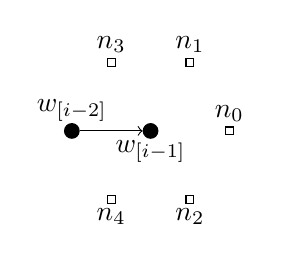
\begin{tikzpicture}
	\fill[shift=(180:1)] (0,0) circle [radius=0.1];
      \fill[shift=(180:0)] (0,0) circle [radius=0.1];
      
      \draw[->] (180:0.9) -- (180:0.1);

	\node[above] at (180:1) {$w_{[i-2]}$};
	\node[below] at (180:0) {$w_{[i-1]}$};
	\node[above] at (0:1) {$n_0$};

	\foreach \theta in {0,60,-60,120,-120}{
   	   \draw [shift=(\theta:1)] (-0.05,-0.05) rectangle (0.05,0.05);
  	}
 	\node[above] at (60:1) {$n_1$};
	\node[below] at (-60:1) {$n_2$};
	\node[above] at (120:1) {$n_3$};
	\node[below] at (-120:1) {$n_4$};
    \end{tikzpicture}
    \caption{$\alpha = 4$: when $w[i]$ is stabilized}
    \label{TTT_a4_lemma_fig}
\end{figure}

\begin{figure}
 \centering
    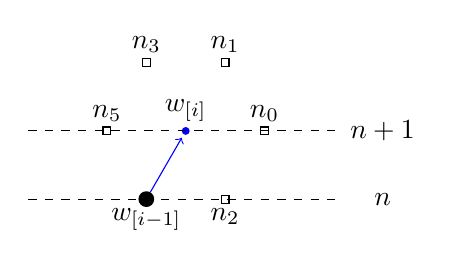
\begin{tikzpicture}
	\fill[shift=(-120:1)] (0,0) circle [radius=0.1];
      \fill[shift=(180:0), blue] (0,0) circle [radius=0.05];
      
      \draw[dashed] (180:2) -- (0:2);
      \draw[dashed, shift=(-60:1)] (180:2.5) -- (0:1.5);
      \draw[->, blue] (-120:0.9) -- (-120:0.1);

	\node[below] at (-120:1) {$w_{[i-1]}$};
	\node[above] at (180:0) {$w_{[i]}$};
	\node[above] at (0:1) {$n_0$};

	\foreach \theta in {0,60,-60,120,180}{
   	   \draw [shift=(\theta:1)] (-0.05,-0.05) rectangle (0.05,0.05);
  	}

 	\node[above] at (60:1) {$n_1$};
	\node[below] at (-60:1) {$n_2$};
	\node[above] at (120:1) {$n_3$};
	\node[above] at (180:1) {$n_5$};
	
	\node at (0:2.5) {$n+1$};
	\node[shift=(-60:1)] at (0:2) {$n$};
    \end{tikzpicture}
    \caption{the first bead out of $\hexagon_{w[-n+1]}^n$}
    \label{TTT_a4_first}
\end{figure}

\end{document}
